%
% University of Berne
%
% Bachelor Thesis Template
% Thomas Kolonko 20.01.2017
%

\documentclass[11pt,a4paper,twoside,hidelinks,]{rvsbachelor}

\usepackage[latin1]{inputenc}
\usepackage{graphicx}
\usepackage{float}
\graphicspath{ {./images/} }
%%%%%%%%%%%%%%%%%%%%%%%%%%%%%%%%%%%%%%%%%%%%

\usepackage[a4paper,twoside]{geometry}

\sloppy

%% Additional packages
%%%%%%%%%%%%%%%%%%%%%%%%%%%%%%%%%%%%%%%

% for source code highlighting
% \usepackage{listings}
% \lstloadlanguages{tcl, Perl}
% \lstset{language=tcl, commentstyle=\it, basicstyle=\tiny, keywordstyle=\bf, breaklines=true, frame=single}

% multiple figures with same general caption
\usepackage{subfigure}
\setcounter{lofdepth}{2}  

% offers more possibilities in captions
\usepackage{caption}

% Commands for package caption
% - caption
\renewcommand{\captionfont}{\small}
\renewcommand{\captionlabelfont}{\bfseries}

% offers rotation of figures, ...
\usepackage{rotating}

% to support correct hyphenaten, add words with -
% \hyphenation{test-case}

% or minimize the occurences of them
%http://tex.stackexchange.com/questions/182569/how-to-manually-set-where-a-word-is-split
\usepackage{microtype}

% If a page has no content, make it an empty page (without page numbers ....)
\makeatletter
\def\cleardoublepage{\clearpage\if@twoside \ifodd\c@page\else
	\hbox{}
	\thispagestyle{empty}
	\newpage
\fi\fi}
\makeatother


% check whether we are running pdflatex
\newif\ifpdf
\ifx\pdfoutput\undefined
\pdffalse % we are not running pdflatex
\DeclareGraphicsExtensions{.eps}
\else
\pdfoutput=1 % we are running pdflatex
\pdfcompresslevel=9     % compression level for text and image;
\pdftrue
\DeclareGraphicsExtensions{.pdf,.png,.jpg}
\fi
\ifpdf
%to make table of contents and index appear in bookmarks
\usepackage{tocbibind}
%refs also as links
\usepackage[pdftex,plainpages=false]{hyperref}
%plainpages=false: enable links although page numbering is reset after title
%backref, pagebackref]{hyperref}
%\usepackage[pdftex]{color}
%\usepackage[pdftex]{thumbpdf}
\else
%url must be escaped. (this works fine in dvi)
\usepackage{url}
\fi


\author{Thomas Kolonko}
\title{Multipath Transmission for Content-Centric Networking in Vehicular ad-hoc Networks}
\date{2017}

\begin{document}
\maketitle
\thispagestyle{empty}
\mbox{}

\newpage
\pagenumbering{roman}
\tableofcontents{}
\listoffigures{}
\listoftables{}
% if you have some code listing, you can include a list of all your listings
% \lstlistoflistings{}



% if you want to thank somebody for the support during your studies make it here
\chapter*{Acknowledgments}
On this page I would like to thank everybody who supported me to write this bachelor thesis.
First I would like to thank my coach Eirini Kalogeiton. She supported me trough the whole process of writing this thesis, spend many hours for pair programming sessions and gave valuable inputs when nothing seemed to work anymore.
After that I would like to thank Prof. Dr. Torsten Braun who allowed me to write this thesis in his research group. I am also very grateful for the resources that were generously provided by the research group of Prof. Braun.

\begin{abstract}
Content-Centric Networking (CCN) is a new network approach based on the information-centric networking paradigm (ICN), which tries to provide a more secure, flexible and scalable network. CCN does not operate on a host-to-host basis but emphasizes the content itself by making it directly addressable and routable. Knowledge of the topology is therefore not required as the routing is based on the names of the content and happens only locally on the intermediate nodes. This allows much more efficient communication in highly mobile and dynamic environments, where no static topology is given, and devices enter and leave a given area very frequently.

\vspace{5mm} %5mm vertical space

In this thesis a new routing strategy for VANET's has been developed in ndnSIM version 2.0 within the ns-3 network simulator. The current implementation supports only routing based on incoming and outgoing faces. Since Wifi and other forms of wireless networking broadcast data by design, a new mechanism has been introduced for forwarding and discriminating by mac addresses. Two new fields have been added to the interest and data packages for original and target mac addresses. FIB tables were extended with the new mac address fields in order to forward the interests to the correct upstream nodes. PIT tables were also extended so that the data could follow the interests way back to the requesting consumer. A new strategy has been implemented for flooding the interest if the FIB entries have not yet been populated with known mac addresses and to forward specifically hop by hop if the FIB entries showed actual intermediate target nodes with lower costs. (TODO: add some info about the multiple netDevices when done)

\vspace{5mm} %5mm vertical space

The scenario was implemented and evaluated using the ns-3 network simulator. Simulation with 100 nodes were conducted for 21 times and ...... (TODO: finish this part as soon as you have some results)

(TODO: CHANGE WORDING from Amadeo14 BEGIN) -> Performance evaluation is carried by means of ndnSIM, the official NDN simulator, that is overhauled for use in realistic wireless ad-hoc environments. Results collected under variable traffic loads and topologies provide insights into the behaviors of both forwarding approaches and help to derive a set of recommendations that are crucial to the successful design of a forwarding strategy for named data ad-hoc wireless networking <- (TODO: CHANGE WORDING from Amadeo14 END)
\end{abstract}

\cleardoublepage
\setcounter{page}{1}	% Reset page numbering to 1
\pagenumbering{arabic}	% Arabic page numbers

% Advice: split up your thesis in multiple files, i.e. one file for one section
\chapter{Introduction}

In the past years, content production and dissemination have both drastically increased. That has led among others to the wide use of Content Distribution Networks (CDN) that tackled the problem of distributing content more efficient and without slowing down main servers. Not only the amount of data has changed, but also the overall mobility has increased exponentially. A commuter on his way to work expects to stream full HD movies on his cell phone or at least listen to Spotify while traveling by train at high speeds. Mobile IP was an attempt to solve some of the issues with high mobility, but the main problem of secure and always active host-to-host connections still remains, and is one of the reasons why the need for a new network architecture becomes more and more pressing.

\section{Motivation}

Vehicular Ad-Hoc Networks (VANETs) are mobile entities that create spontaneously wireless networks for the exchange of data. This exchange can be for a very short or a prolonged time. It depends on a broad variety of applications from very basic information about a moving car in front or rather weather information from a central server. Information dissemination of messages in certain areas play an important role to VANETs and question arise how to best solve the issues that arise with no static topology, fast moving entities like cars, drones, bikes or even trains that can be used for propagation of data over long distances to place unreachable by other means. New forwarding strategies need to be implemented in order to get information about possible content sources and how data can reach fast moving entities. Problems like intermittent links and no static host to host connections play an important role among other problems like security and privacy, content caching and efficiency.

Named Data Networking (NDN) is an implementation of Information-Centric Networking (ICN) and tries to solve the above mentioned problems through a paradigm. It is built upon the same innovative concepts as other ICN implementations. These are among others the named content and the routing by that name as in-network caching of data. This is in contrast to the current Internet architecture that is based on host to host communication. This makes NDN with ndnSIM (it's simulator) very appealing for mobile ad-hoc environments with no static topology whatsoever.

\section{Study Subject}

The goal of this thesis is to implement a forwarding strategy that can be used in a mobile ad-hoc environment and tested against different scenarios for performance metrics. The implementation will be done in NS-3 and ndnSIM which is a simulator based in C++. First, some research is needed to find out what has been implemented already in ndnSIM. If there are some strategies already, the main goal will be to implement a forwarding strategy that will outperform the default strategy. The scenario will be based on VANETs. Nodes will be used as mobile entities that move and interact with each other. The scenario will start with no prior knowledge of the topology and as data passes through the network routes and nodes will be discovered. This information will be used to further improve the dissemination of information.

\section{Outline}

The remainder of this thesis is organized as follows. Chapter 2 explains shortly why a paradigm shift takes place from host-based networking to content-centric networking, explains what Content-Centric Networking (CCN) is and why it could outperform the TCP/IP model. It will contain and go into related work already done on this subject. Chapter 3 explains ndnSIM and it's current implementation of the forwarding mechanism and the strategy as of version 2.0. In chapter 4 the design and the implementation of the forwarding strategy are described. In addition, the modifications that have been performed on ndnSIM together with the algorithm for the forwarding strategy are presented. In Chapter 5 the results are evaluated and discussed. Finally, a conclusion of the thesis is offered in Chapter 6.
\chapter{Related Work}

Todays use of the Internet is heavily based on content dissemination of all kinds of media like audio and video. TV-Shows, clips and tutorials on Youtube, podcasting for educational purposes like on Coursera need to be distributed around the globe. Popular TV-Shows are being distributed globally within the first few hours after being telecast to the audience through p2p networks. When a video clip goes viral millions of requests for the content are made from all over the world. In 2008 alone 500 exabytes were created and today's number is a multiple of that [TODO: reference]. This became possible, since computers and computing devices got so inexpensive that almost anybody can afford them. Limited storage on clouds is given free to all users by many providers. When the Internet was invented, there were only a few computers and few resources like tape storage devices, archives or computing power distributed geographically. A client requested some specific information or resources from a specific destination which needed to be known to the client. The client was connected through TCP/IP to the server, and after the connection was established and possibly secured, the transfer of the information needed by the client could start. Host-centric networking was very reasonable at that time, but the Internet evolved towards content-dissemination and with it's evolution the need for new and more efficient solutions.

\vspace{5mm} %5mm vertical space

TCP/IP is no longer best suited for todays use of the Internet. One of the main reasons is that a TCP/IP connection is established between two machines and requires it to be active at all times. For content dissemination a mechanism that supports multipoint to multipoint connections that do not have to be active at all times might be much better. Another reason is that a client often does not know where to get some specific information from (and doesn't really care) but knows exactly what it wants. Therefore a paradigm shift from host-centric networks started to evolve towards content-centric networks.

\newpage
\section{Named Data Network / Content Centric Networks}

Information-centric networking (ICN) is a possible answer to today's problems with TCP/IP architecture. ICN originated as a possible new paradigm for the future internet to improve on scalability, reliability and efficient content distribution. One of the many ICN architectures is content-centric networking (CCN) originally introduced by Van Jacobson. It is being continuously researched around the globe and one initiative trying to implement CCN is Named Data Networking (NDN) project.

\vspace{5mm} %5mm vertical space

In CCN the content is made directly addressable and routable by name. An Interest (request by a client) is sent out and routed according to it's name until it reaches some endpoint that is able to respond with Content Objects to that Interest. Some of the main goals of CCN is better utilization of the bandwidth by increasing throughput and decreasing network traffic, better security, availability, flexibility and scalability of the networks. Better utilization of the bandwidth can be achieved by multicasting the same content to several endpoints and not re-unicasting the same content over and over again through the same channels near the content source. Also content caching in intermediate nodes reduces the strain on bandwidth and increases overall efficiency. Better security is achieved by hashing and signing the content itself instead the point-to-point connection between two hosts. (TODO: why is encrypting data not make it more private? No key -> no content) Encrypting the data leads to more privacy within the Internet and could substitute many current access policy patterns used by servers and webpages. (TODO: don't understand why not) Better availability and flexibility are intrinsically given by content caching. Better scalability is achieved by not needing pre-planned structures like CDN's and P2P networks. Data is not only kept at the content producer but everywhere along the route if necessary.

\begin{figure}[H]
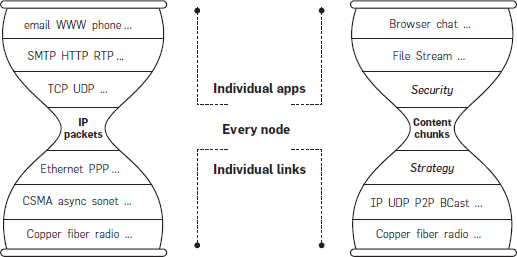
\includegraphics[scale=0.6]{chapter-2/NetworkStack}
\centering
\end{figure}

In Figure 1 the IP and CCN protocol stacks are compared to each other. Both protocol stacks are built in a modular fashion that makes the architecture very flexible and scalable. The thin waste of the TCP/IP protocol stack consists of IP packages that have a source and a destination address. This Network Layer is kept very simple and it makes only very weak demands on layer 2. This thin waist in TCP/IP protocol stack (\emph{where}) is replaced in CCN with a content layer (\emph{what}) that describes what the package is and has even fewer demands on the lower layer, keeping much of the advantages from IP. Lower layers of the CCN protocol stack are responsible for the routing, encoding and decoding of the information while the higher layers consist of security and interpretation of the information. Because of the modularity CCN can be implemented on top of IP.

\vspace{5mm} %5mm vertical space

Two big differences of TCP/IP and CNN are the strategy layer and the security layer. The strategy layer is responsible for all dynamic routing decisions based on the name and the strategy. The strategy can be a different one for different namespaces. E.g. an emergency message could be always broadcasted according to it's name. The Security layer differs from the TCP/IP protocol stack, since the content chunks are signed and encrypted themselves, contrary to TCP/IP, where the connection is secured.

\subsection{CCN/NDN Node Model}

In CCN there are no clients and servers anymore but \textbf{consumers} and \textbf{producers}. Consumers request some information by sending out an \textbf{interest}. This interest packet consists of a content name, some selectors and a nonce. The interest is being forwarded according to the node's strategy until it reaches a node that can satisfy it. If a node can satisfy the received interest, it will respond with a \textbf{data} package consisting of the same content name as the interest, a signature, signed info and the data. The data will be sent back towards the consumer. The node having the requested information is called producer (it generates the data). Interests and data are received and sent out through interfaces which can be network or application interfaces. (TODO: is an intermediate node that does NOT generate it but supports it also a producer???).

\begin{figure}[H]
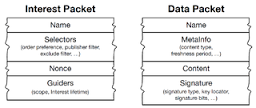
\includegraphics[scale=1]{chapter-2/InterestAndData}
\centering
\end{figure}

The most important data structures for routing the interest to the producer and the data back to the consumer are called the pending interest table (PIT), the forwarding information base (FIB), and the content store (CS). A PIT entry is also needed to detect loops among other things. If an interest arrives at the node having the same content name as a previous interest, it's nonce will be checked against the PIT entry's nonce. If both nonces are the same the interest has been looped otherwise another consumer requested the same data.

\subsubsection{PIT}

The Pending Interest Table (PIT) keeps track of all the interests that have been forwarded towards potential content sources. It also keeps track of all incoming and outgoing faces of the specific interests (multiple in-faces and out-faces reflect the multipoint to multipoint characteristics of CCN). If a second interest with the same content name but different nonce arrives at the node, the incoming face will be added to the already existing PIT entry of the previously forwarded interest. The interest will not be re-forwarded and shortly after dropped. It won't be deleted right away since a looped interest is identified by it's nonce. When an interest reaches a content source or a producer data is send back. It follows the the breadcrumbs (faces) left in the PIT entries to find it's way back to the consumer. The PIT entries are deleted shortly after the requested data has been sent downstream.

\subsubsection{CS} 

The Content Store (CS) is located within the intermediate nodes. It is a cache of data packages that have passed this node and have been saved for later use. That is a critical advantage over TCP/IP where data packages are meant only for point to point delivery. It depends on the implementation of the CS to decide which packages (solicited and unsolicited) should be saved to the cache and how they should be replaced if the cache is full. Current implementation focus mainly on Least Recently Used (LRU) and Least Frequently Used (LFU) replacement strategies. The CS needs to be searched before the interest is handed off to the forwarding strategy.

\subsubsection{FIB}

The Forwarding Information Base (FIB) is used by the strategy to forward interests upstream towards potential producers or intermediate nodes, that have cached the requested data. Every interest that needs to be forwarded will be matched against the FIB entries. If an entry is found (longest prefix match) then the interest will be send upstream to the outgoing faces. If there is no match the interest can be broadcast or dropped. The FIB is always checked last if there is no PIT entry (it has not yet been forwarded or it has been already satisfied) and there is no CS data that can satisfy the interest directly.

\subsection{Forwarding of an Interest}

Interests are forwarded based on the content name and the implemented strategy on all intermediate nodes. The above discussed tables are used for deciding if and how to further process the interest. The strategy is only responsible for forwarding the interests towards content sources or producers. The Data coming back follows the path of the interest back to the consumer.

\begin{figure}[H]
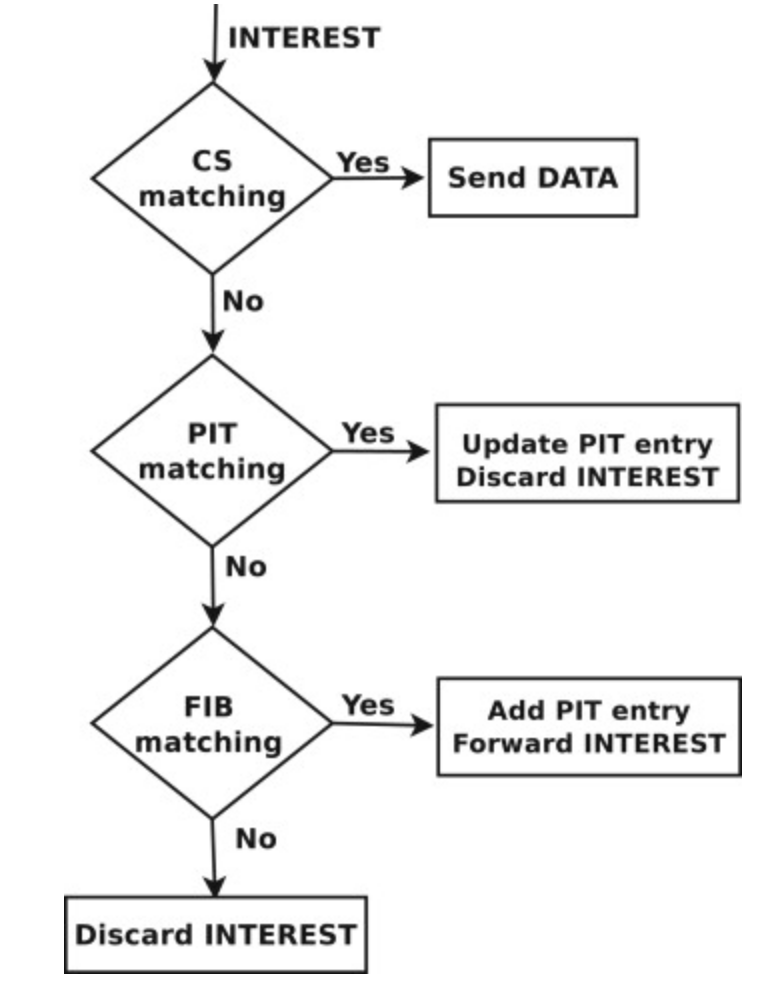
\includegraphics[scale=0.4]{chapter-2/SimpleInterestForwarding}
\centering
\end{figure}

When an interest arrives at some intermediate node the first thing to do is to check if there is already some data in the content store (CS). If the interest can be satisfied by some cached data the data is send downstream towards the consumer and the interest is dropped (not further processed). If the CS has no data with the same content name as in the interest, the PIT entries are checked. If a PIT entry already exists for the interest the node has already requested the data and is awaiting it. The incoming face(s) are added to the existing PIT entry and the interest is dropped. If a PIT entry does not exist yet and no cached data can satisfy the interest, the node needs to forward the interest upstream towards a potential content source. The strategy checks the FIB entries for a longest prefix match. If an entry is found a new PIT entry has to be created with the content name of the interest, it's incoming face and outgoing face (from the FIB). The interest is then forwarded according to the FIB and the strategy.

\vspace{5mm} %5mm vertical space

Sending Data downstream to the original requester is straightforward since no special routing is required. The Data follows the path of the interest left within the PIT entries (in-face(s) of the interest at that node). 

\subsection{Transport and Routing}

As mentioned above the "content chunks" layer in the CCN protocol stack makes even weaker demands on the lower layers then the IP layer makes on layer 2. It operates on unreliable, best-effort packet delivery services in potentially highly dynamic and mobile environments. Interests and Data packages are expected to get lost and/or corrupted. In CNN the strategy layer of the intermediate nodes is responsible to resend the interest if within the timeout no data has been received. The strategy layer knows which outgoing faces were used and what the timeout was, therefore able to adjust the parameters for a retransmission. The same is true for the strategy layer of the consumer. If it does not receive any data back within a given timeframe, it too, will resend (possibly rebroadcast) the interest.
Flow control can be managed by the consumer in terms of how many interests can be sent out before having received the first data packages back. It is also managed on a hop-by-hop basis. Each intermediate node decides when to retransmit an interest due to loss or corrupted data coming back. The buffer for the interests is the PIT whereas the buffer for the data passing downstream to the consumers is the CS. There is no need for special congestion control techniques. (TODO: find the reference for that)

\subsection{Sequencing}

One of the big advantages in CCN over the host-to-host based TCP/IP approach is that the data in transition can be used many times by many different consumers requesting the same data possibly far away from the original producer. That leads to the problem of uniquely identifying the data in a self explanatory way. Consumers must be able to deterministically construct a name for the data without having previously seen it. Hierarchical names that reflect the content and the organizational structure of their origin are very well suited to solve that problem. Since the naming is absolutely irrelevant for the network (TODO: find the reference for that), applications can choose a naming that fits their need best. For example, to get the segment 34 of a video version 2 by group A of the University of Bern the name could be: \textbf{/unibe.ch/group/A/videos/introduction.mpg/\_v2/\_s32}\\
This name can be aggregated with more components if needed by the application or network. It only needs to adhere to previously specified rules.


\subsection{Network Security}

CCN digitally signes and encrypts the content itself and not the connection over which it travels. TCP/IP needs to secure the connections which in turn must link the content to the server infrastructure. To trust a content the user must fetch it from it's original source making it very difficult to cache popular content and make it available to other users. For a rich and robust content-based security model the consumer must be able to assess the integrity (content is not corrupted), pertinence (what question does it answer) and provenance (who claims this is an answer). TCP/IP can only provide weak integrity through a checksum and only implicit pertinence and provenance through securing the host to host channel and therefore trusting the source and destination addresses. CNN on the other hand transparently provides then content name and therefore the meaning of the content which satisfies pertinence. Through public key signatures the consumer and any node in between can check the content's authenticity, therefore verify integrity and satisfy provenance.
Content Protection and Access Control could be solved solely by encrypting the content with different keys. No trusted servers or directories would need to enforce complicated access policies on the filesystem. Expensive authentication services like SWITCH AAI could be saved. If for example certain documents within a database should be only readable by a certain group of people these documents could be simply encrypted while still accessible to everyone. Only the people with the correct key could encrypt it and use it.
Network security is improved against many classes of network attacks. Every node can possibly (if the resources allow it) check the integrity of the data and cache it for further use. There is no single host that provides the data, therefore hiding content from consumers is very difficult.
DDoS attacks with data packages are not really a problem since every node can ignore unsolicited data coming in. If resources allow it, the node can simply store it in CS and mark it as unsolicited. If the space runs low on the CS these data packages will be removed first. No propagation of unsolicited data takes place since no PIT entries exist for the data. DDoS attacks therefore would have to be done through interests. If the prefix stays the same the PIT entry get's updated for every new interest, but no forwarding takes place. If the prefix changes constantly the strategy has many means to take action like limiting the rate of the interests with certain prefix patterns or lower prioritization of interests that result in data coming back. 

\newpage
\section{VANETs}

Vehicular ad hoc network's (VANETs) operate in very dynamic and mobile environments under possibly poor and intermittent connectivity. To the few static roadside unites (RSU) there are many devices ranging from trackers and phones on pedestrians other vehicles like cars, motorcycles or drones to airplanes and satellites as shown in Figure (TODO: X).

\begin{figure}[H]
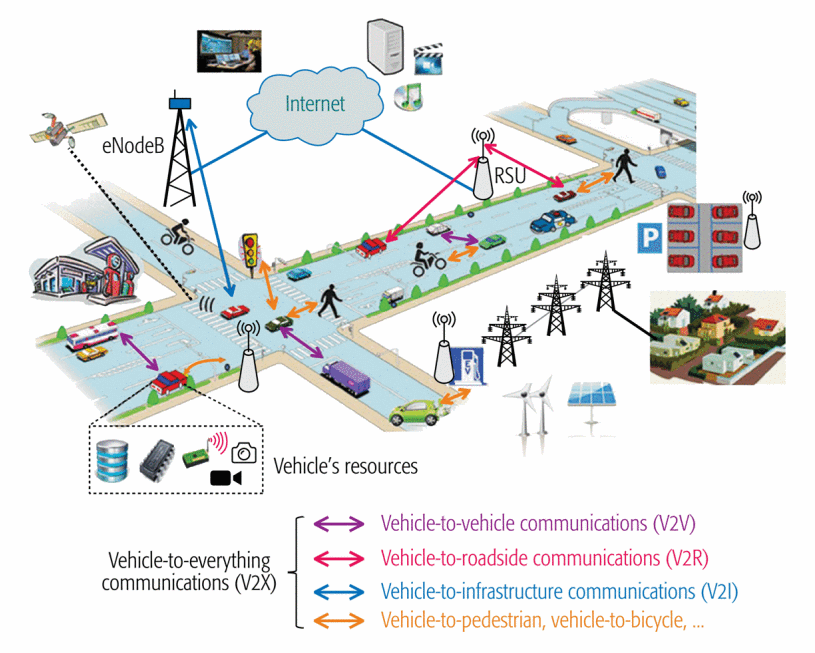
\includegraphics[scale=0.4]{chapter-2/VANETecosystem}
\centering
\end{figure}

In such dynamic and mobile environments the TCP/IP based approach that focuses on the source and destination and their secured connection quickly becomes a burden. Dynamic name-to-IP resolutions are difficult to do and infer a high management overhead. Keeping the connection up in urban areas where signal propagation is obstructed frequently can quickly become a challenge. Mobile IP is a workaround for this problem but does not solve the issue really. The CCN approach on the other hand seems to be very well suited for such ecosystems where the focus lies on the information itself (trusted road safety information for a specific area) and not on the identity of the host (other vehicles, RSU, Internet) the data might have originated from. With in-network caching the CCN approach also tackles the problem of poor signal strength and intermitted connectivity within a very heterogenous network system. A vehicle can even store information and propagate it to a otherwise disconnected area through a \emph{store-carry-and-forward} mechanism. The multipoint to multipoint characteristics already mentioned before allows to aggregate the same interests (maps, safety warnings, road condition, congestion warnings....) and multicast the arriving data through different faces and different channels back to the consumers simultaneously.

\vspace{5mm} %5mm vertical space

There are two main routing schemes for VANET's. In the \emph{proactiv} scheme the content providers advertise periodically in order to keep the FIB entries updated with fresh routing information. In the \emph{reactive} scheme no advertisement by the content providers is done and the FIB's are populated based on interest flooding. Flooding-based discovery seems to be better suited for VANET's since periodical FIB updates on all intermediate nodes incur a high and mostly unnecessary cost on the network. An interest is able to find it's way quickly to some node having a copy of the data or the producer itself. Collision avoidance and packet suppression is done on lower layers, although packet suppression will be done in the forwarder module in ndnSIM (see chapter 3).
Caching policies in VANET's differ slightly from regular CCN use since the vehicles are moving fast into and out of regions relevant to the data. Data about possible congestion gets outdated pretty quickly so do often warnings of any kind. Further the question arises if unsolicited data should be cached into CS and if yes, under which conditions and for how long? As mentioned before vehicles could link otherwise disconnected areas, but in that case the data naming should be clear or that specific intent.

\vspace{5mm} %5mm vertical space

While the vehicles and devices are getting smarter and are being equipped with ever more sensors, it is expected that they will produce a huge amount of data. Most of it will be aggregated and logged, some of it will be available for distribution some of it should remain private. There are many open questions how to best support the information flow given the networks capacity. Although not originally intended by ICN the intermediate nodes could be included into in-network processing of the data like filtering useless data or aggregating redundant information.









\chapter{ndnSIM}

Named Data Networking (NDN) is a newly proposed Internet communication paradigm that tries to keep most of the well accepted and tested TCP/IP Internet architecture (as shown in \ref{fig:NetworkStack}), while evolving the thin waist introducing many new features \cite{ndn17}. These features differ in fundamental ways from a point-to-point communication architecture and need to be simulated extensively under constantly changing parameters and implementations \cite{Ajunwadkar14}.

NdnSIM is an open source simulator for NDN networks within the existing NS-3 simulator framework. Its main goals are to facilitate experimentation inside the research community and make all basic NDN protocol operations accessible and therefore changeable like routing, data caching, packet forwarding and congestion management \cite{mastorakis16}. Packet-level interoperability with CCNx implementation is given in order to support traffic measurements, traffic traces and analysis tools between CCNx and ndnSIM. Large-scale simulations should be supported and made easy to set up through helper classes. Helper classes automate the repetitive creation of single entities like nodes and set them up in a standardized way. Therefore, the simulator has been implemented in a very modular fashion making it very easy to modify, replace or re-implement specific components like the FIB, PIT or forwarding strategy. Replacing components have minimal or no impact on other components, as long as they adhere to the modules API's and other components they interact with \cite{Afanasyev16}.

\newpage

\section{Design overview}

NS-3 and ndnSIM both follow a philosophy of maximum abstraction for all modeled components making experimentation on one hand very fine-grained and on the other hand very isolated and decoupled from the rest. The NDN core protocol stack can be installed on every simulated network node in a consistent manner through helpers, that take care of all the parts that need to play together like the inter-node communication with installed applications through their respective application faces.

\vspace{5mm} %5mm vertical space

\begin{figure}[H]
  \centering
  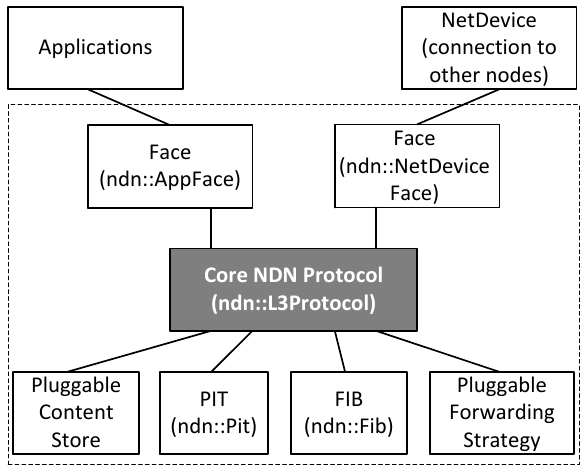
\includegraphics[scale=0.4]{chapter-3/ndnSIMcomponentAbstraction}
  \caption{Basic component abstractions in ndnSIM \cite{afanasyev12}}
  \label{fig:ndnSIMcomponentAbstraction}
\end{figure}

\vspace{5mm} %5mm vertical space

The basic component abstractions are seen in figure \ref{fig:ndnSIMcomponentAbstraction}. The core NDN Protocol is the ndn::L3Protocol that receives Interest and Data packets from upper and lower layers through the corresponding faces. As of ndnSIM version 2.0 there are two distinct faces: the application face (ndn::AppFace) is responsible for inter-node communication between the application and the node itself while the net device face (ndn::NetDeviceFace) is responsible for inter-network communication with different nodes. Other faces for different purposes are expected to be added by the core developer or the community as needed. The CS (ndn::ContentStore) is an abstraction for in-network caching of Data and can easily be omitted or replaced by another implementation of a different storing policy. The PIT (ndn::Pit) abstracts the Data structure that is responsible for logging all received Interests with their nonce and incoming faces while the FIB (ndn::Fib) abstracts the Data structure to guide the strategy in Interest forwarding. The Strategy (ndn::ForwadingStrategy) is responsible for implementing how Interests and Data are forwarded. That includes lookups in the content store for cached Data, in PIT for already forwarded Interests and in FIB if both previous searches didn't yield any matches. Each action in the forwarder of the strategy is represented as a virtual function in the forwarder header class and can be overwritten.

\subsection{Face Abstraction}

The face abstraction plays an important role in the overall modularity of the NDN simulator by acting as an interface, therefore, making ndnSIM design independent from any underlying transport layers. All communication between application, the NDN core protocol and other nodes with the L3 protocol happens through faces that take care of any needed conversion.

\vspace{5mm} %5mm vertical space

\begin{figure}[H]
  \centering
  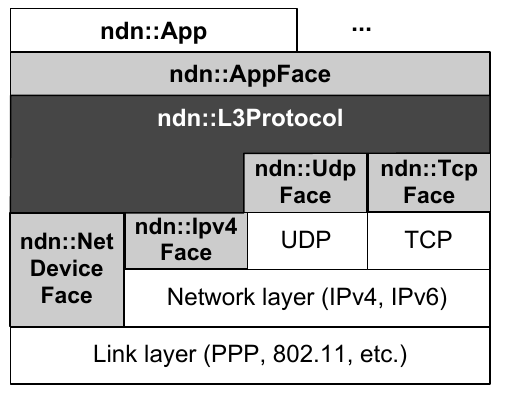
\includegraphics[scale=0.4]{chapter-3/CommunicationLayerAbstraction}
  \caption{Face abstractions around ndn::l3Protocol \cite{afanasyev12}}
  \label{fig:CommunicationLayerAbstraction}
\end{figure}

\vspace{5mm} %5mm vertical space

As shown in \ref{fig:CommunicationLayerAbstraction} the application can communicate with ndn::L3Protocol through the AppFace whereas for inter-node transmission it depends on the transmission protocols which faces need to be used. TCP and UDP have their respective ndn::UdpFace and ndn::TcpFace. IPv4 and IPv6 also have their own ndn::Ipv4Face making it particularly easy to implement the NDN architecture on top of IP or even TCP/IP. If NDN needs to be implemented without TCP/IP protocol it can communicate directly with the link layer through the ndn::NetDeviceFace.

\subsection{Content Store Abstraction}

The CS is crucial for the NDN Internet architecture as it caches Data for later use in potentially all the intermediate nodes. It can do rudimentary error recovery and multicast the data asynchronously downstream to the requesters. The replacement policy determines what data is saved into cache and how it gets replaced or deleted after a certain time. Currently implemented versions of the CS support Least Recently Used (ndn::cs::Lru), First In First Out (ndn::cs::Fifo) and a Random Replacement Policy (ndn::cs::Random). Each implementation is based on a dynamic trie-based Data structure with hash-based indexing as are the PIT and FIB implementations.

\subsection{Pending Interest Table (PIT) Abstraction}

The PIT Data structure keeps information about each forwarded Interest. Each PIT entry is uniquely identified by the content name of the Interest. It holds a list of all incoming faces on which the Interest was received and a list of all outgoing faces that the Interest has been forwarded to. The arrival and expiration time are also kept in order to retransmit a lost Interest. The nonce of an Interest is a randomly generated number that is attached to the Interest and identifies the Interest in order to avoid loops. Nonce and Interest name uniquely identify the Interest. Different consumers issuing the same Interest will very likely have different nonces. In that case, no loop is detected and the incoming face is added to the already existing PIT entry. If the same nonce and Interest are received again, the Interest has looped and should be dropped.

\vspace{5mm} %5mm vertical space

\begin{figure}[H]
  \centering
  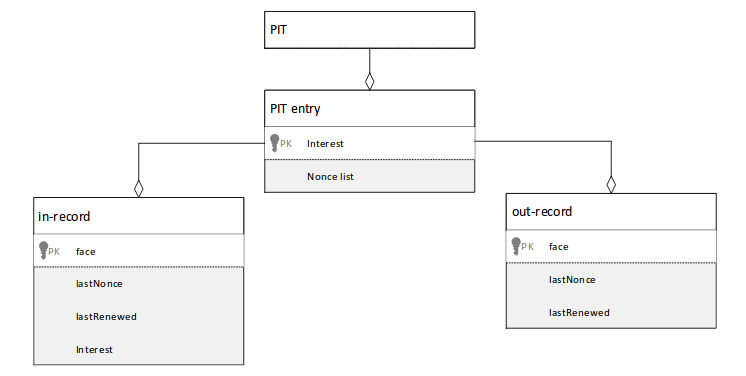
\includegraphics[scale=0.4]{chapter-3/PITdataStructure}
  \caption{PIT Data structure \cite{Afanasyev16}}
  \label{fig:PITdataStructure}
\end{figure}

\vspace{5mm} %5mm vertical space

Figure \ref{fig:PITdataStructure} shows the different PIT classes and how they relate to each other. There are also two additional timers on every PIT entry that are not explicitly shown here. The \emph{unsatisfy timer} is the lifetime of an Interest and counts down. If it reaches 0 the PIT entry has expired and needs to be forwarded again. The \emph{straggler timer} starts counting down as soon an Interest got rejected or satisfied. The straggler timer gives the node the time to detect further loops by the satisfied or rejected Interest still floating within the network. Also, Data plane measurements of returning data might require to still finish obtaining data points just after that event. Deleting the PIT entry immediately, there would be no means to detect loops and acquire valuable measurements \cite{Afanasyev16}. After the straggler timer runs out the PIT entry is deleted. The PIT abstraction provides basic functions to insert, lookup, delete PIT entries and get measurements if necessary.

\newpage

\subsection{Forwarding Information Base (FIB) Abstraction}

The FIB guides the forwarding strategy in making decisions about Interest forwarding. It is similar to an IP's FIB but contains name prefixes instead of IP prefixes and holds several interfaces (out-faces) therefore enabling multicast forwarding. The faces are ordered according to their cost (routing metric) putting the cheapest connections at the beginning of the list. The lookup is performed on the content name prefixes. The longest prefix match yields the requested FIB entry with its outgoing face(es).

\vspace{5mm} %5mm vertical space

\begin{figure}[H]
  \centering
  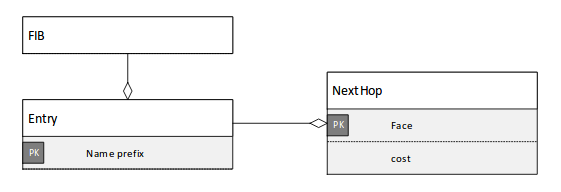
\includegraphics[scale=0.4]{chapter-3/FIBdataStructure}
  \caption{FIB Data structure \cite{Afanasyev16}}
  \label{fig:FIBdataStructure}
\end{figure}

\vspace{5mm} %5mm vertical space

As shown in Figure \ref{fig:FIBdataStructure} each FIB entry that has been identified by longest-prefix match has an aggregated collection of NextHops. The NextHop collection must be non-empty and for every NextHop there is one outgoing face towards a possible content source. There may only be one NextHop with a specific face id. The FIB abstraction provides basic insertions, deletions, and exact match operations.

\subsection{Forwarding Strategy Abstraction}

NdnSIM's modular architecture allows experimenting with different types of forwarding strategies without having to adapt any core components. The forwarder class interacts with the strategy and has the following important functions:

\begin{itemize}
\item \emph{onIncomingInterest}: checks for localhost violations and if the Interests have looped. Then the function inserts or updates the PIT, resets its timers and looks if the Interest can be satisfied by cached data.
\item \emph{onContenStoreMiss}: if there is no data to satisfy the Interest, the strategy is called.
\item \emph{onOutgoingInterest}: this function is called by the strategy and forwards the Interest to the outgoing faces.
\item \emph{onIncomingData}: checks for localhost violations and if there are any PIT entries for that data. If there are no PIT entries the data is dropped, otherwise, the Data packet will be handed on to the onOutgoingData function.
\item \emph{onOutgoingData}: forwards the data downstream towards the content requester.
\end{itemize}


The strategy is called on three occasions. The first time from the forwarder::onContentStoreMiss(), when the decision has to be made how to forward the Interest upstream. The second time from the forwarder::onContentStoreHit() to decide how to proceed with a satisfied Interest. And the last time from the forwarder::onIncomingData()

\vspace{5mm} %5mm vertical space

The strategy has one important function:

\begin{itemize}
\item \emph{afterReceiveInterest}: it receives the Interest and the corresponding FIB and PIT entries from the forwarder and decides how to forward them further and through which faces.
\end{itemize}


\section{Simulation Environment}

The NS-3 simulator supports several simulation environments. In this thesis, NS-3 PyViz was used as a live simulator \cite{pyviz}. PyViz also has an interactive console that visualizes the connections between the nodes of the simulation. It also can be used to debug the state of the running object, show PIT and FIB entries in live and where packets are being dropped.

\vspace{5mm} %5mm vertical space

\begin{figure}[H]
  \centering
  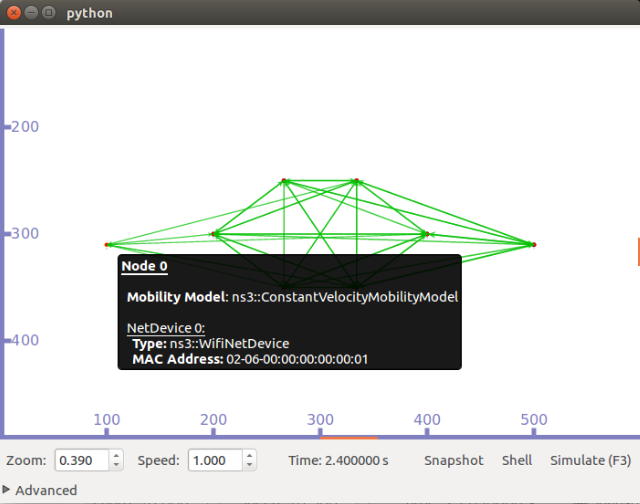
\includegraphics[scale=0.4]{chapter-3/Simulation}
  \caption{Simulation of a possible scenario}
  \label{fig:Simulation}
\end{figure}

\vspace{5mm} %5mm vertical space

Figure \ref{fig:Simulation} shows a current scenario in development. Zoom and speed can interactively be adjusted. The simulation can be started and paused at any time. Node-specific information can be shown while hovering over the node. Traffic between the nodes is visualized by green lines. The current utilized bandwidth is mentioned just above the traffic lines in a live simulation.

\vspace{5mm} %5mm vertical space

\begin{figure}[H]
  \centering
  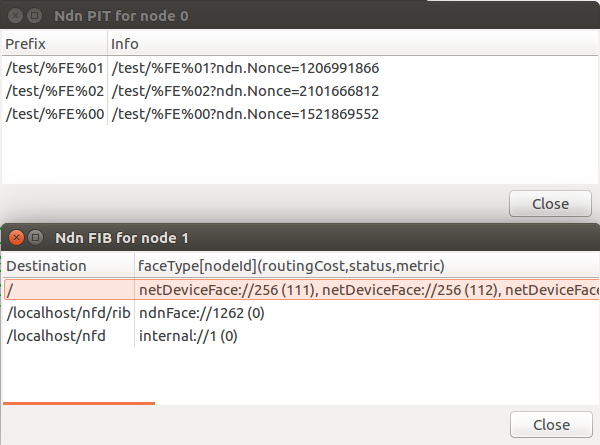
\includegraphics[scale=0.4]{chapter-3/PITandFIBvis}
  \caption{PIT and FIB entries in real time}
  \label{fig:PITandFIBvis}
\end{figure}

\vspace{5mm} %5mm vertical space

Figure \ref{fig:PITandFIBvis} shows all the PIT and FIB entries in real time. Face id's with the corresponding face type are also shown for easier debugging purposes.

\section{Forwarding by the NDN Forwarding Daemon (NFD)}

\vspace{5mm} %5mm vertical space

All the above mentioned modular components and abstractions are implemented and coordinated by the NDN Forwarding Daemon (NFD), which is a network forwarder that implements and evolves with the NDN protocol. NFD is responsible to correctly forward Interest and Data packets, maintain all basic Data structures like CS, PIT and FIB, and implement the packet processing logic. Management interfaces are used by NFD to configure, control and monitor the different components.

\vspace{5mm} %5mm vertical space

Packet processing in NFD is accomplished through forwarding pipelines and forwarding strategies. A forwarding pipeline is an aggregation of different steps that are applied on a packet or a PIT entry. Forwarding pipelines are triggered by specific events like the reception of an Interest, detection of a loop, of when an Interest is ready to be forwarded further, etc. A forwarding strategy is attached at the beginning or the end of a pipeline and supports it with information about how and when to forward the Interest. Figure \ref{fig:PipelinesAndStrategies} shows the interactions between forwarding pipelines and strategies. For the thesis, relevant pipelines will be shortly described.

\vspace{5mm} %5mm vertical space

\begin{figure}[H]
  \centering
  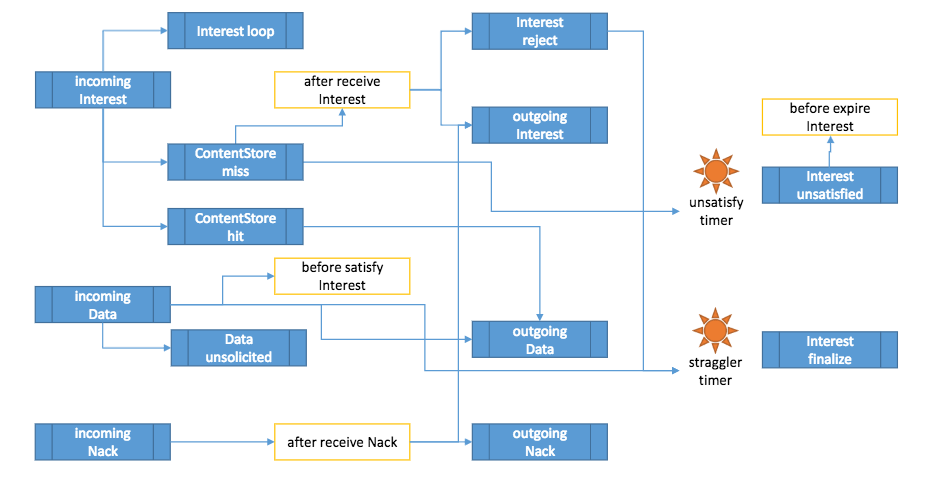
\includegraphics[scale=0.4]{chapter-3/PipelinesAndStrategies}
  \caption{Pipelines and Strategies, white boxes are decision points inside the strategy while blue boxes represent the different pipelines \cite{Afanasyev16}}
  \label{fig:PipelinesAndStrategies}
\end{figure}

\vspace{5mm} %5mm vertical space

Forwarding pipelines operate on Interests, Data and nacks (negative acknowledgments send downstream to inform about the failure to satisfy a particular Interest). After a pipeline has finished it's processing, the packet is handed off to another pipeline or to a decision point inside the strategy until all processing is finished. NFD uses three main forwarding paths:

\begin{itemize}
\item \emph{Interest Processing Path}
\item \emph{Data Processing Path}
\item \emph{Nack Processing Path}
\end{itemize}

The first two paths will be explained further. The nack processing path has not yet been implemented in ndnSIM 2.0 and is under active investigation, therefore it will not be explained.

\subsection{Interest Processing Path}

The Interest processing path consists of the following pipelines:

\begin{itemize}
\item \emph{incoming Interest}: Interest has been received through a face and is ready to be processed by the forwarder
\item \emph{Interest loop}: loop has been detected and Interest needs to be dealt with
\item \emph{content store miss}: incoming Interest cannot be satisfied by the content store
\item \emph{content store hit}: incoming Interest can be satisfied by CS and does not need further forwarding 
\item \emph{outgoing Interest}: Interest is made ready and sent out
\item \emph{Interest reject}: strategy rejects Interests according to PIT entries
\item \emph{Interest unsatisfied}: processing unsatisfied PIT entries before timeout
\item \emph{Interest finalize}: deletion of PIT entries
\end{itemize}

\subsubsection{Incoming Interest Pipeline}

After receiving an Interest packet through a face implemented in \texttt{Face::onReceiveInterest} the Interest is forwarded to the incoming Interest pipeline that is implemented in \texttt{Forwarder::onIncomingInterest} method. The input parameters to this method are the Interest itself and a reference to the face it was received on. Figure \ref{fig:IncomingInterestPipeline} shows all the steps taken within the pipeline.

\vspace{5mm} %5mm vertical space

\begin{figure}[H]
  \centering
  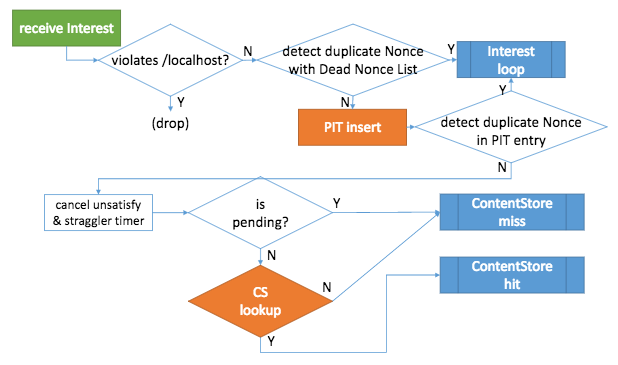
\includegraphics[scale=0.5]{chapter-3/IncomingInterestPipeline}
  \caption{Pipelines and Strategies, white boxes are decision points inside the strategy while blue boxes represent the different pipelines \cite{Afanasyev16}}
  \label{fig:IncomingInterestPipeline}
\end{figure}

\vspace{5mm} %5mm vertical space

The following is a short step by step description of the pipeline in figure  \ref{fig:IncomingInterestPipeline}:

\begin{enumerate}
\item An Interest reaching the node through a non-local face is not allowed to have the \texttt{\\localhost} prefix since this prefix is reserved for localhost communication only. This check is necessary because Interests with the \texttt{\\localhost} prefix can be used to configure the node and make unwanted changes. The compliant forwarder has no reason to send such an Interest to a non-local face.
\item Next the name of the Interest with its nonce is checked against the dead nonce list. That happens before the PIT entry is created for the incoming Interest (supplements the regular nonce checking through PIT entries). If the tuple of Interest and nonce have been processed already, the incoming Interest has been looped and will be handed off to the Interest loop pipeline.
\item Using the name and the selectors of the Interest the PIT is searched for matches. If no match can be found a new PIT entry is created, otherwise an existing PIT entry is updated with the new information mainly the inFace and timers. In Figure \ref{fig:SimpleInterestForwarding} of chapter 2 the CS was checked first, then the PIT was searched and created if necessary. NFD has a slightly different approach. It is expected that the CS will be much larger than the PIT. A search in the CS may take much longer than a PIT lookup, and if a pending Interest is present the CS lookup can be omitted saving time and resources.
\item The nonce of the Interest is checked against the nonces in the PIT and if a loop or multi-path arrival is detected the Interest will be handed off to the Interest loop pipeline. If no loop or multi-path arrival is detected the forwarding process is continued.
\item Since a new valid Interest arrived and the PIT entries got updated, the current unsatisfy timer (fires when the PIT entry expires) and the straggler timer (fires when PIT entry is no longer needed after it has been satisfied or rejected) are canceled.
\item This step checks if the Interest is pending (if the PIT entry has already another in-record from the same or different face).
\item If there is no PIT entry a CS lookup is needed in order to satisfy the Interest (ContentStore hit) or forward it (ContentStore miss). If there is already a pending Interest the CS lookup has been done already on a previous Interest that led to a PIT entry since no match could be found.
\end{enumerate}

\subsubsection{ContentStore Miss Pipeline}

If the ContentStore lookup in \texttt{Forwarder::onIncomingInterest} doesn't yield any data that can satisfy the Interest, the content store miss pipeline is called. This pipeline is implemented in \texttt{Forwarder::onContentStoreMiss} and the parameters for this method are the Interest packet, the incoming face and the PIT entry. The validity of the Interest has been checked already and it needs to be forwarded by taking the following steps:

\begin{enumerate}
\item In the incoming Interest pipeline a PIT entry was created already. Now the in-record with its incoming face needs to be added to the PIT entry and if it already exists then the in-record with its face is updated. The expiration counter is set to the value of the Interest's field \texttt{InterestLifetime}.
\item The PIT entry's unsatisfy timer is set. It will expire as soon as all in-records of this entry have expired and hand control off to the Interest unsatisfied pipeline.
\item The content store miss pipeline then decides which strategy to use and forwards the Interest with its incoming face and PIT entry to the chosen strategy for further processing.
\end{enumerate}

The incoming Interest pipeline has finished.

\subsubsection{ContentStore Hit Pipeline}

If the ContentStore lookup in \texttt{Forwarder::onIncomingInterest} does yield a match, the content store hit pipeline is called through its implementation in \texttt{Forwarder::onContentStoreHit}. The parameters include the Interest packet, incoming face, the PIT entry and the Data. The straggler timer is being set since the Interest is about to be satisfied. After that, the Data is handed off to the outgoing data pipeline.

The incoming Interest pipeline has finished.

\subsubsection{Outgoing Interest Pipeline}

The \texttt{Forwarder::onOutgoingInterest} method implements the outgoing Interest pipeline. It is entered from the \texttt{Strategy::sendInterest} or a child of the Strategy class that overrides the method. The parameters are the PIT entry, the outgoing face and a \texttt{wantNewNonce} boolean that signalizes that a new nonce is needed for the Interest. As mentioned above the PIT entry holds a reference to the Interest and therefore the Interest packet is not in the parameters list. Figure \ref{fig:OutgoingInterestPipeline} illustrates the outgoing Interest pipeline.

\vspace{5mm} %5mm vertical space

\begin{figure}[H]
  \centering
  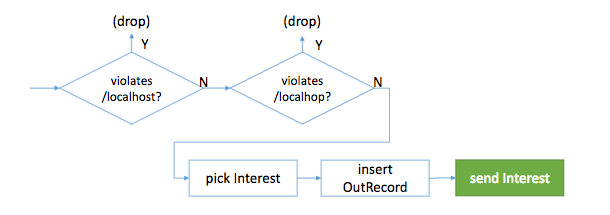
\includegraphics[scale=0.5]{chapter-3/OutgoingInterestPipeline}
  \caption{Outgoing Interest pipeline \cite{Afanasyev16}}
  \label{fig:OutgoingInterestPipeline}
\end{figure}

\vspace{5mm} %5mm vertical space

\begin{enumerate}
\item First localhost and localhop violation is checked. Interests with a /localhost scope are not permitted to be sent out through non-local faces. Interests with a /localhop scope are permitted to be sent out through a non-local face only if the PIT entry has one or more in-records with that has a local face stored in it.
\item The Interest is picked from the PIT entry and saved to a local variable.
\item If the \texttt{wantNewNonce} flag is set, the Interest is copied and a new nonce is attached to it. This is necessary when the node needs to retransmit the Interest. If the Interest wouldn't receive a new nonce it would be recognized as a looped Interest and dropped immediately.
\item An out-record is created in the PIT entry and add an out-face to it. If an out-record with the same out-face already exists, the entry gets refreshed by the \texttt{InterestLifetime} value.
\item The Interest is forwarded upstream via out-face.
\end{enumerate}

\subsection{Data Processing Path}

The data processing path consists of the following pipelines:

\begin{itemize}
\item \emph{incoming Data}: incoming Data are processed
\item \emph{Data unsolicited}: unsolicited (not requested) Data are processed
\item \emph{outgoing Data}: Data is forwarded downstream
\end{itemize}

\subsubsection{Incoming Data Pipeline}

 \texttt{Face::onReceiveData} fires when a Data arrives at a face. It triggers the  \texttt{Forwarder::onData} which calls \texttt{Forwarder::onIncomingData} with the incoming face and the Data as parameters.
The following figure \ref{fig:IncomingDataPipeline} summarizes the steps taken by this pipeline:

\vspace{5mm} %5mm vertical space

\begin{figure}[H]
  \centering
  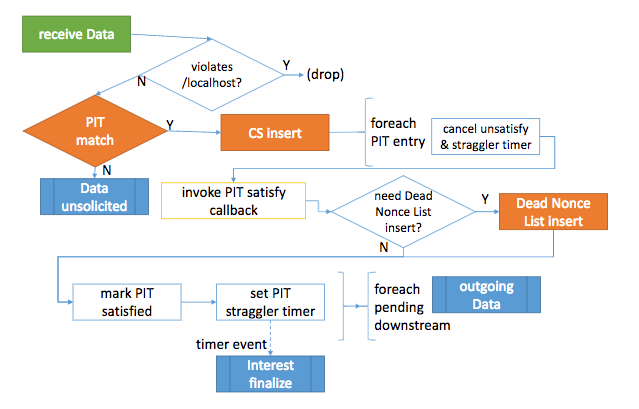
\includegraphics[scale=0.5]{chapter-3/IncomingDataPipeline}
  \caption{Incoming Data pipeline \cite{Afanasyev16}}
  \label{fig:IncomingDataPipeline}
\end{figure}

\vspace{5mm} %5mm vertical space

\begin{enumerate}
\item Like with the incoming Interest pipeline the /localhost scope needs to be checked. Data may not contain the prefix /localhost when coming from a non-local face.
\item The incoming Data needs to be checked against the PIT entries to find out if it is solicited or unsolicited. The Data is unsolicited if no matching PIT entry is found. In this case, it is forwarded to the next pipeline: Data unsolicited.
\item If one or more PIT entries have been found the Data is solicited and therefore inserted into the CS. How the Data is processed in the CS is up to the policies defined in the content store.
\item The unsatisfy and straggler timers for all matched PIT entries need to be canceled since the Interest is being satisfied.
\item The responsible strategy is determined and triggers the method \texttt{Strategy::beforeSatisfyInterest}. By default, it is empty in ndnSIM 2.0 and can be implemented by a custom strategy overriding the method.
\item The nonce of the Data is added to the dead nonce list for further loop detection since Interest and Data could still be floating inside the network. This is necessary because the next steps delete the corresponding in- and out-records of the PIT entry and the nonce would be lost. 
\item The PIT entry is marked satisfied. All in-records and out-records (corresponding to the incoming face of the Data) are being deleted.
\item For every pending downstream the Data is handed off to the next pipeline, the outgoing data pipeline, with its corresponding face. NFD takes care that the Data is handed off only once for every distinct downstream, even if several PIT entries are found.
\end{enumerate}

\subsubsection{Outgoing Data Pipeline}

The outgoing data pipeline is implemented in \texttt{Forwarder::onOutgoingData} and can be called from two different pipelines. If the incoming Interest pipeline found a CS match, the Data is fetched and passed to \texttt{Forwarder::onOutgoingData} with the corresponding out-face (the Interest's in-face in the PIT entry). If the incoming data pipeline found one or more PIT matches, the Data and out-face are passed to this method.

This pipeline has three steps:

\begin{enumerate}
\item The localhost scope is checked. Data with the prefix /localhost are not permitted to be sent out through a non-local face.
\item This step is reserved for traffic management and traffic shaping but not implemented in ndnSIM 2.0 yet.
\item The Data packet is sent out through it's out-face.
\end{enumerate}



\chapter{Design and Implementation}


\section{Problem Description}

\section{Multipath approach}
\chapter{Evaluation}

The evaluation is conducted on several independent scenarios. As mentioned in chapter 1 the thesis relies on four subtasks that need to be solved. First the forwarding should rely on MAC addresses of the WiFi network interface (also called net devices) and not the different faces. The second subtask is to implement a forwarding strategy that can be used with the MAC addresses. The third part is to add mobility to the intermediate nodes while the fourth part is to improve on the forwarding strategy. Every scenario is evaluated and compared to the ndnSIM's multicast strategy \texttt{nfd::fw::MulticastStrategy}, which has been implemented in ndnSIM version 2.0 as basic multicast strategy. The thesis will refer to this multicast strategy as the base strategy or only base. It basically receives an interest and forwards it to all available faces of the node except the receiving one. The newly implemented forwarding strategy will often be referred to as the new strategy or the improved strategy.

To achieve comparability the scenario and trace-files are copied into a clean base installation of ndnSIM version 2.0. All parameters are kept equal. Then it is run once on the clean installation and once on the improved one. In the first scenario the implementation of the mac addresses and the forwarding mechanism is tested and evaluated. In the second scenario mobility is introduced with changes to the strategy. The different scenarios are tested for interest/data ratio, latency, congestion and number of distinct routes, although distinct routes do not exist in the already existent multicast strategy. It is introduced as part of the thesis for the new implementation.

\section{Evaluation environment}

All tests are run on the ns-3 network simulator with ndnSIM version 2.0. Different trace files are used for the two distinct scenarios. NS2 Mobility Helper uses these trace files and adds movement to the nodes. As Wifi standard 802.11a was used, which means each node has a transmission range of approximately 120 meters in open space \cite{wifi80211a} . For the propagation delay \texttt{ns3::ConstantSpeedPropagationDelayModel} was used and for the propagation loss \texttt{ns3::ThreeLogDistancePropagationLossModel} and \texttt{ns3::NakamiPropagationLossModel} were used. Interest lifetime is set to 4 seconds and the retransmission timeout to 500ms. Data packet size is 1200kb.

\section{Results for a static 8 nodes scenario}

The first scenario is a static 8 node scenario with one consumer on the left and one producer on the right. 6 intermediate nodes are placed in between as seen in figure \ref{fig:scenario1}. Every node has 3 net devices with distinct MAC addresses. They allow on one hand to send and receive simultaneously, while extending on the multi-path idea. The paths are determined by the FIB entries that have been configured with MAC addresses from data being forwarded downstream. Therefore a first segment of an interest can be requested through the first net device. The second segment through the second net device and the third segment through the third net device. The fourth segement would be sent again through the first net device. That is achieved by a static counter and a modulo operation leading to different routes.

\begin{figure}[H]
  \centering
  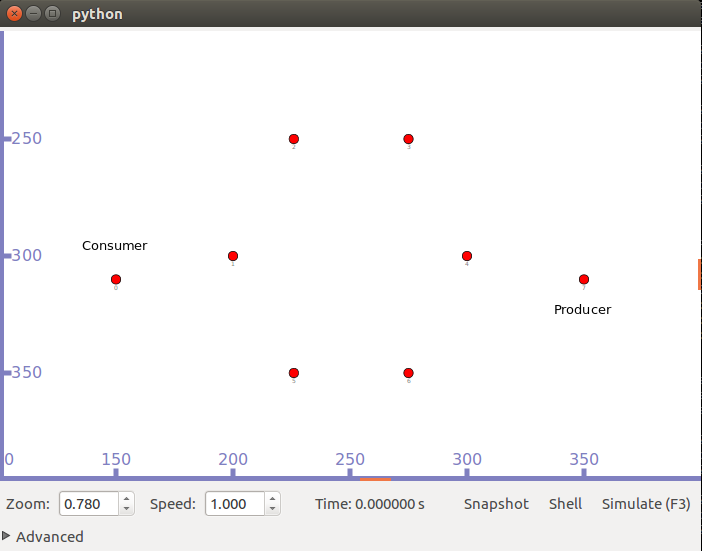
\includegraphics[scale=0.5]{chapter-5/scenario1}
  \caption{Basic static scenario with 8 nodes, 1 consumer and 1 producer}
  \label{fig:scenario1}
\end{figure}

The runs have been conducted for 100, 200, 300 and 600 seconds each. The consumer was configured to sent out interests at a frequency of 3 interests per second. For the ratio, received data over send interests only distinct packages were counted. Retransmissions were ignored. The average latency was measured in nanoseconds, as the time difference of the interest leaving the consumer and the corresponding data package being received at the consumer, added together and divided by all successful interest requests.

\begin{figure}[H]
  \centering
  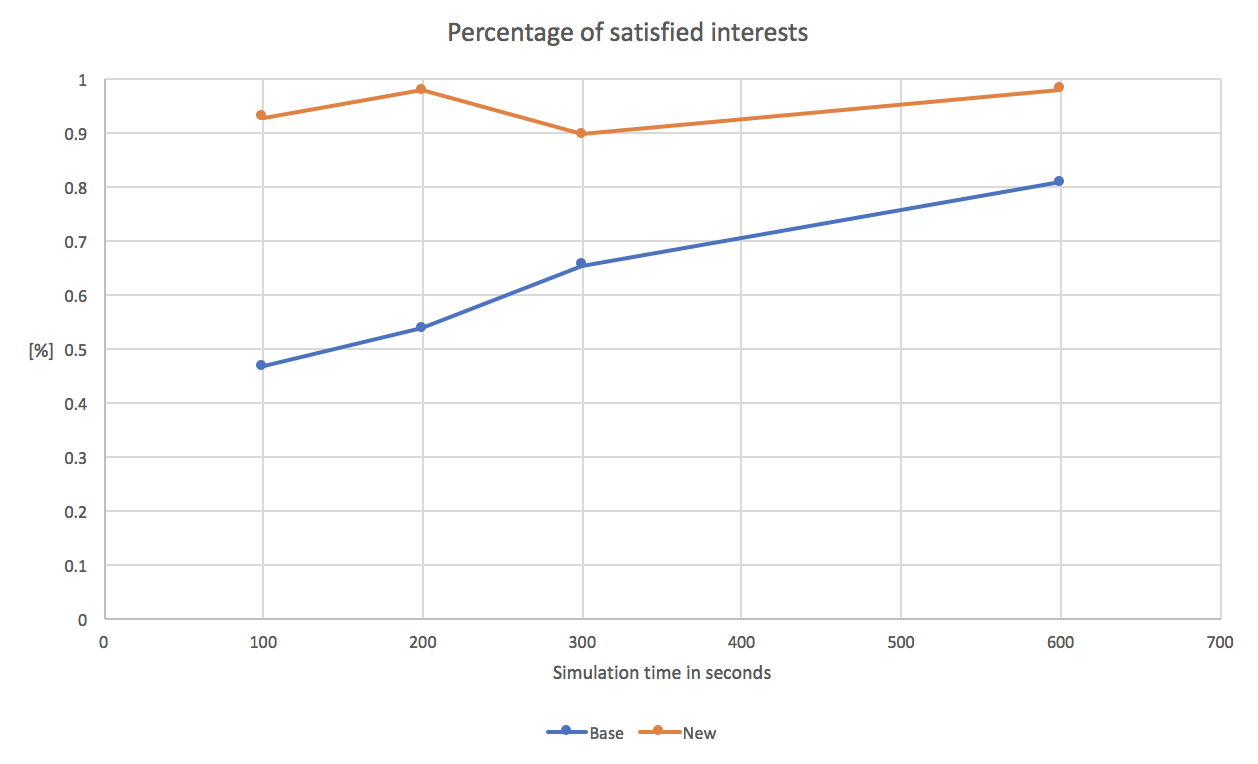
\includegraphics[scale=0.6]{chapter-5/staticS1ratio}
  \caption{Satisfaction ratio at different simulation times for both implementations}
  \label{fig:staticS1ratio}
\end{figure}

Figure \ref{fig:staticS1ratio} compares the ratio of satisfied interests (interests send / data received back) over simulation time. A better ratio has been observed for the new implementation at all simulation times. The difference is biggest at a run time of 100 seconds. At a run time of 600 seconds the difference has been reduced to 0.171. That is due to the amount of interests and data being in transition. As the number of satisfied interest constantly rises over time, the unsatisfied interest will not keep getting more since retransmissions will be made after new interests are introduced to the network.

Figure \ref{fig:staticS1iod} shows that the ratio alone (as shown in figure \ref{fig:staticS1ratio}) does not make any statement about the amount of the interests sent towards a potential content producer and the amount of received data. With the base implementation there is not much gain with increased simulation time whereas with the new implementation the gain nearly doubles. The reason for that observation is explained with congestion. Broadcasting the interest at each node leads to an exponential increase in the packages being retransmitted within the network leading to congestion, loss of packets and retransmissions. The new implementation floods the network only with the first interest and uses configured routes for all further interests leading to much less traffic. Retransmissions have been observed at the consumer and although the new implementation has fewer retransmissions (around 15 percent) it is not very significant and they happen on a much higher transmission rate. It can be expected that the retransmission rate is strongly correlated with the retransmission timer in the consumer and the lifetime of the interest itself.

\begin{figure}[H]
  \centering
  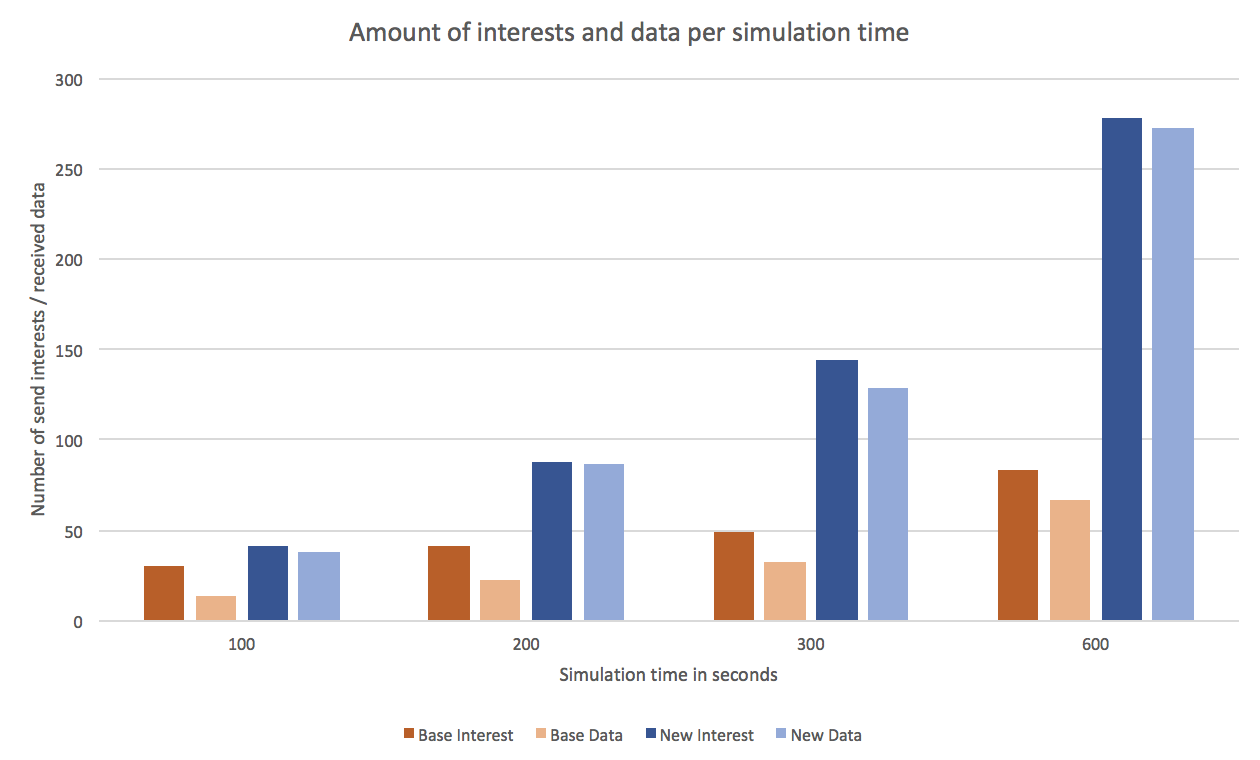
\includegraphics[scale=0.6]{chapter-5/staticS1iod}
  \caption{Number of sent and received packages over simulation time}
  \label{fig:staticS1iod}
\end{figure}

Figure \ref{fig:staticS1latency} shows how the latency changes with the simulation time and chosen implementation. As expected from \ref{fig:staticS1iod} the latency increases significantly with congestion and retransmissions in the base implementation of the multicast strategy. In the first 100 seconds it already reaches 40 seconds which multiplies by 3 at 600 seconds. The new implementation has a much lower latency, starting with around 11 seconds for the first 100 seconds of the simulation. Then increases slightly till around 15 seconds for 600 seconds of simulation. That also shows that congestion and retransmission stay constant for the new implementation.

\begin{figure}[H]
  \centering
  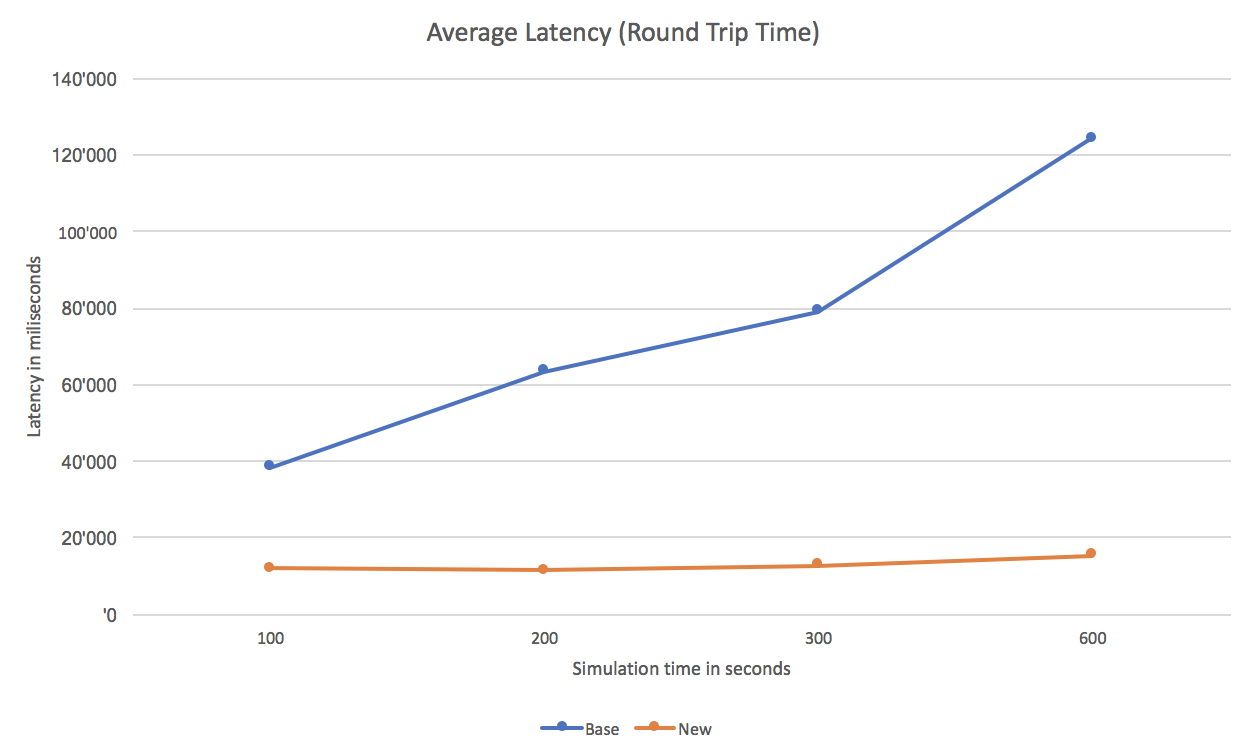
\includegraphics[scale=0.6]{chapter-5/staticS1latency}
  \caption{Latency of both implementations over simulation time}
  \label{fig:staticS1latency}
\end{figure}

The implementation has been tested with overhearing of data coming back and adding the route to the FIB entries but with a higher cost. If the data was intended for the receiving node, the node added or updated the FIB with the new information and attached cost 111 to this specific next hop. The number 111 was randomly chosen and represents a relative low cost. If the data was only overheard (unsolicited) a FIB entry was updated or created with cost 222 instead of ignored and dropped immediately to save resources. The results were slightly worse than the above proposed implementation, but still much better than the base one.

\vspace{5mm} %5mm vertical space

Since one to three new FIB entries were added to every node, an additional approach was to test, if instead of broadcasting or forwarding the interest to only one next hop, better results could be achieved by forwarding the interest to two or three distinct next hops. This yielded again worse results and lead to the above proposed implementation.

\vspace{5mm} %5mm vertical space

One problem with more than one valid FIB entry of next hops was, that the main routes remained the same over the simulation. Instead of alternating between possible next hops only the first one was chosen and the interest forwarded to. Incrementing each cost by one and sorting the FIB's next hops did increase the number of different routes taken. The next hops within the FIB entry were selected in alternating fashion. Unfortunately that did not improve the overall performance. It decreased it despite having more routes to chose from. The reason for this behaviour is how ndnSIM translates FIB next hops cost into transmission time. The lower the cost the more reliable and faster the interest is forwarded. For example setting the cost to 50 after reaching 150 while incrementing all forwarded FIB next hops by one led to significantly better results then looping the cost from 250 to 150. Since that is true for both scenarios equally, it has not been further investigated.

\section{Results for dynamic 16 nodes scenario}

For the dynamic scenario 8 further nodes were introduced. All 14 nodes have been randomly scattered between the consumer and the producer. Random movement was added to the trace file by changing direction and speed of every intermediate node at 5 second intervals. The net devices remain to be three. Retransmission time is set to 500 milliseconds, while the interest lifetime also remains at 4 seconds. 

Figure \ref{fig:scenario2} shows the topology at the beginning of the simulation. The consumer and producer are marked in the figure, and remain static. Only intermediate nodes move in a random manner at different speeds. The distance between consumer and producer as been increased to about 450 meters.

\begin{figure}[H]
  \centering
  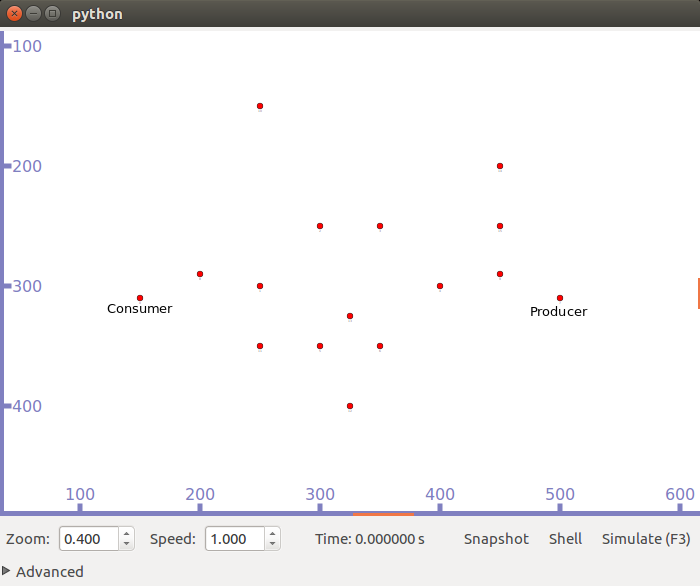
\includegraphics[scale=0.4]{chapter-5/scenario2}
  \caption{Ad-hoc scenario with 16 nodes and movement, 1 consumer and 1 producer}
  \label{fig:scenario2}
\end{figure}

For the static scenario it was sufficient to keep the configured routes constant and not alternate through the intermediate nodes quite that often. On this scenario though, by moving intermediate nodes, the strategy may possibly lead to losing the connection altogether (if the nodes move too far away). The base implementation of ndnSIM does not have this problem since it has no specific routes to follow and basically broadcasts the interest all over again using the next best node available. The trace file was randomly generated in order to give a realistic scenario and the above problem can be seen around simulation time: 200 seconds in figure \ref{ig:scenario2extended}. This problem is also noticed in the numeric data.

\begin{figure}[H]
  \centering
  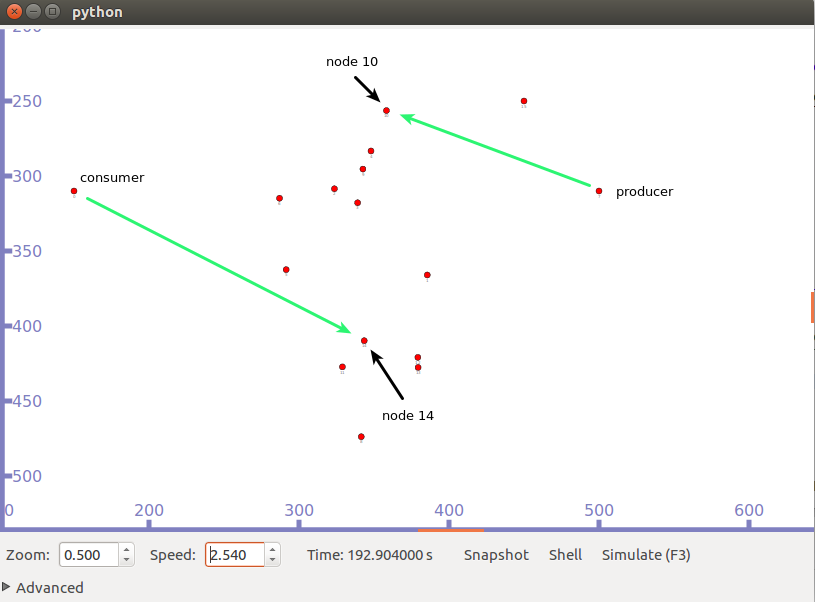
\includegraphics[scale=0.4]{chapter-5/scenario2extended}
  \caption{Node 10 is one of the producer preferred nodes while node 14 is one of the consumer preferred nodes.}
  \label{fig:scenario2extended}
\end{figure}

To counter the aforementioned problem, the interest is forwarded to three FIB next hops (instead of only one) and making the strategy multicast to three nodes upstream the default. Sending the interest to three MAC addresses increases robustness at the cost of generating more traffic, but overall leading to much better results without congesting the network.

Figure \ref{fig:scenario2ratio} shows the ratio of send interest packages over satisfied ones. The new implementation starts from 71.8\% satisfaction rate for the first 100 seconds of simulation and goes up to almost 90\% for the 600 seconds simulation. The ndnSIM base implementation starts lower, but as time passes by, the interests get satisfied through broadcasting and the satisfaction rate rises up to 74.3\%.

\begin{figure}[H]
  \centering
  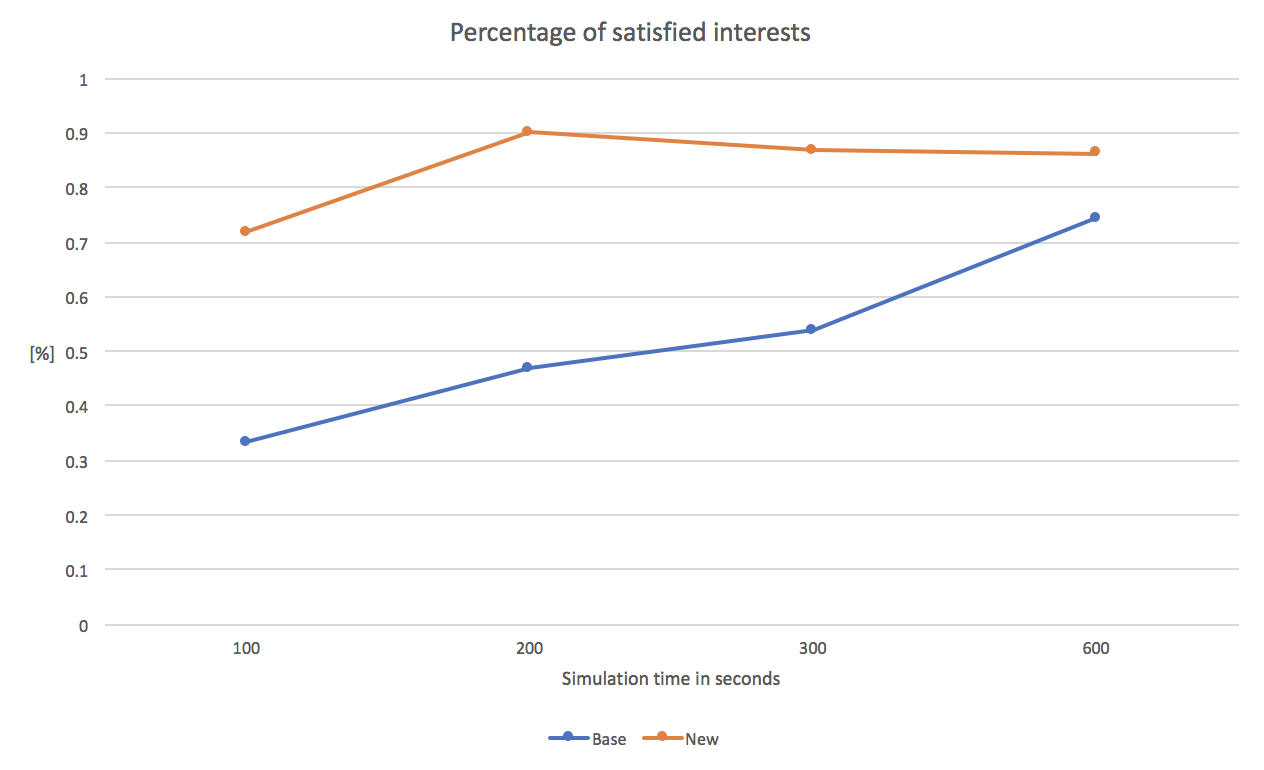
\includegraphics[scale=0.6]{chapter-5/scenario2ratio}
  \caption{Satisfaction ratio at different simulation times for both implementations with mobility}
  \label{fig:scenario2ratio}
\end{figure}

Like in the static scenario it is important to look at the overall throughput and set the satisfaction ratio into context of send and satisfied interests. Figure \ref{fig:scenario2iod} shows the base implementation in brown colour. The dark bar shows the interests send upstream towards a potential content producer, while the lighter bar shows the satisfied interests. The ratio obtained in \ref{fig:scenario2ratio} is seen once again by comparing the bars of one colour per simulation time to each other. The new implementation has not only a better ratio but also is able to send and receive more data. The reason is that the nodes are targeted specifically by the mac address and don't congest the network even if send to three upstream addresses.
The new implementation sends 39 interests out and receives 28 data that satisfy the interests in the first 100 seconds of the simulation. The next 100 seconds roughly doubles the interests being sent and satisfied, whereas the next 100 seconds result in a decrease of newly satisfied interests. That problem was described above and can be seen figure \ref{ig:scenario2extended}. Different trace-file led to different results and whenever a clustering of the intermediate nodes was observed the successfully sent out and satisfied interests also slowed down. The clustering issue is also a problem for the ndnSIM base implementation strategy, but preferred nodes by FIB entries only pose a problem to the new implementation that needs further attention.

\begin{figure}[H]
  \centering
  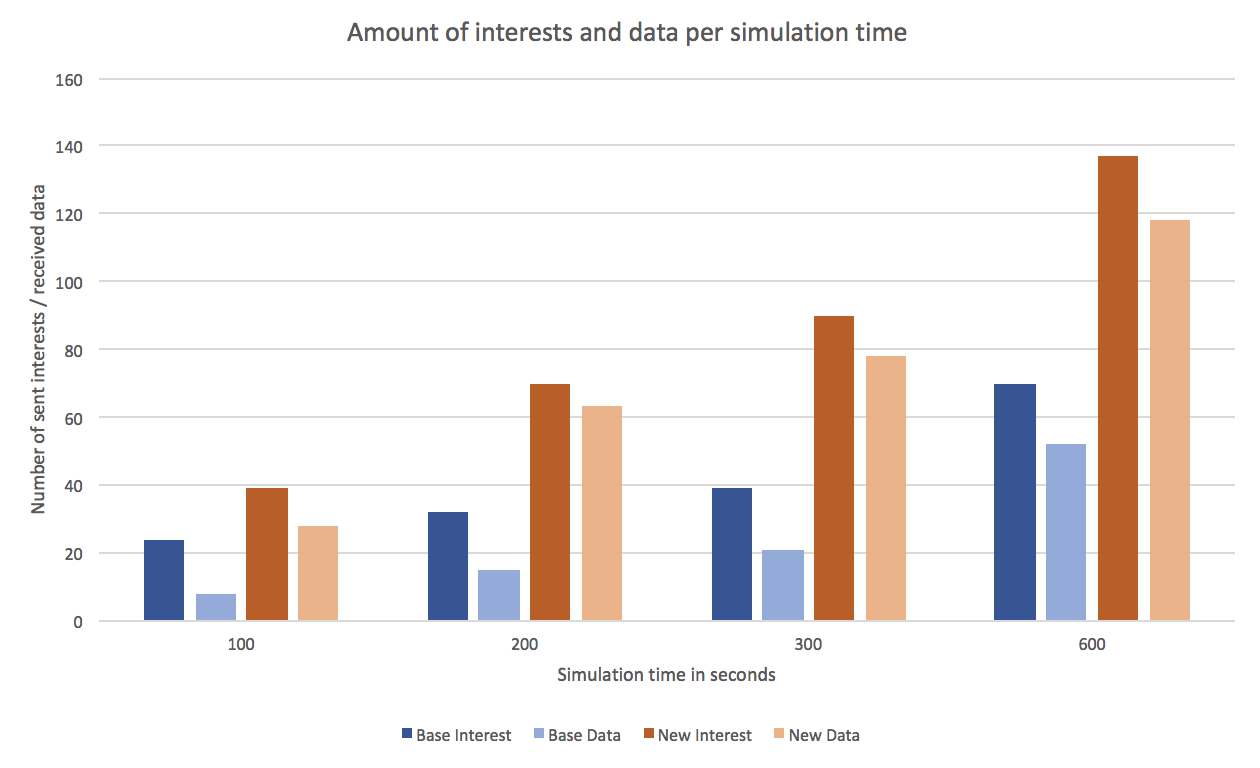
\includegraphics[scale=0.6]{chapter-5/scenario2iod}
  \caption{Number of sent and received packages over simulation time}
  \label{fig:scenario2iod}
\end{figure}

Figure \ref{fig:scenario2latency} shows the observed latency for both implementations. As expected the latency is significantly better with the new implementation, although it is longer, due to increased number of nodes and more distance between the consumer and the producer. As the unsatisfied interests are retransmitted the latency increases over time.

\begin{figure}[H]
  \centering
  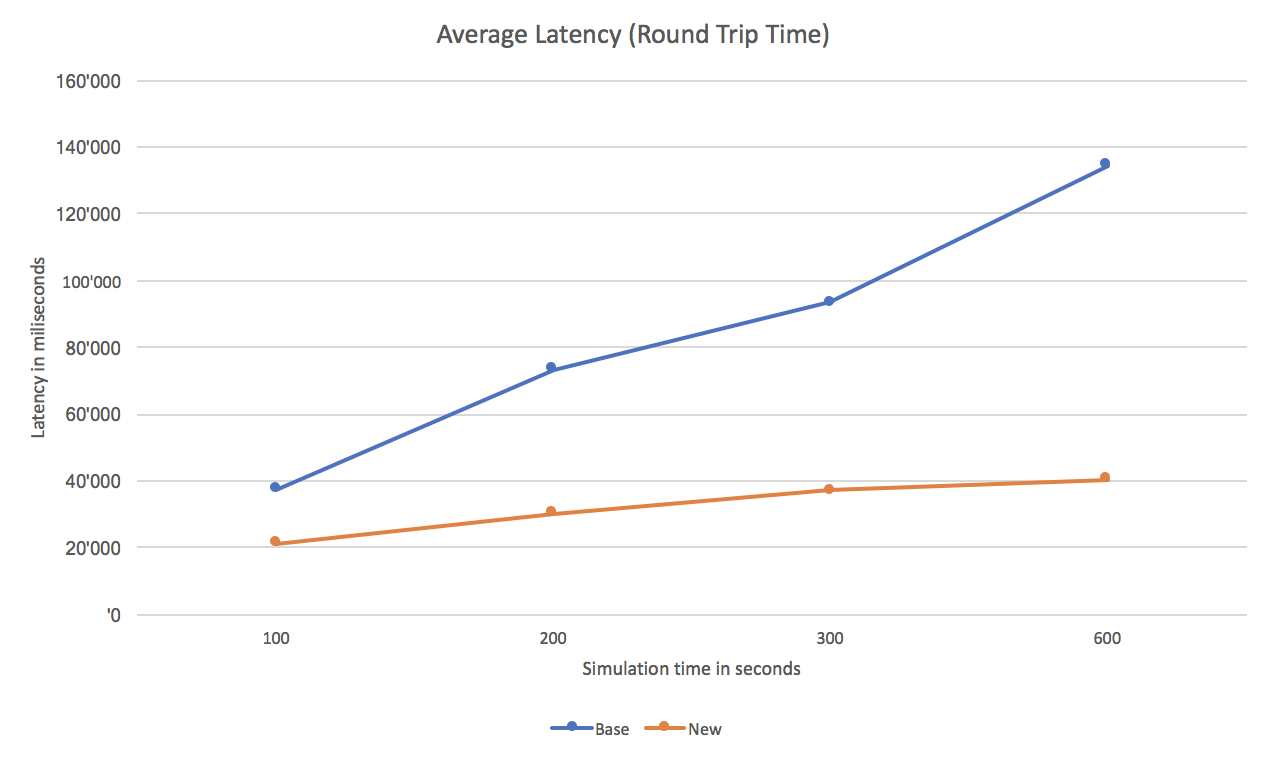
\includegraphics[scale=0.6]{chapter-5/scenario2latency}
  \caption{Latency of both implementations over simulation time}
  \label{fig:scenario2latency}
\end{figure}

In the static and dynamic scenarios the latency time is around 20 seconds, which is too high for real time applications. But can be used well in background processes, like downloading maps, weather forecast or entertainment media.

As an attempt to solve the problem mentioned in figure \ref{fig:scenario2extended} overhearing of unsolicited data was implemented. Different combinations have been tried with overhearing and dropping of unsolicited data. Overheard data could be used to add new FIB next hops of potential next hops otherwise not known and then be dropped or processed further. Overhearing data did yield many more next hops within the FIB entry, but didn't result in better performance. Incrementing the cost at every successful transmission led to overheard FIB entries having similar costs like the originally intended routes mixing them up. This also led to worse results and will need further investigation into this topic on how exactly increment and decrement the cost according to some defined metric and how to separate the overheard routes from the originally intended ones.



\chapter{Conclusion}


\section{Summary and Conclusion}

\section{Future Work}
\chapter{Appendix}




\begin{thebibliography}{99}

\bibitem{jacobson09}
  Van Jacobson, Diana K. Smetters, James D. Thornton, Michael Plass, Nick Briggs, Rebecca Baynard,
  \textit{Networking Named Content},
  Parc, Paolo Alto, 2009
  
\bibitem{ndn17}
  "Named Data Networking: Motivation \& Details", March, 2017. [Online]. Available: {https://named-data.net/project/archoverview}

\bibitem{Ajunwadkar14}
  Dnyanada P. Arjunwadkar
  \textit{Introduction of NDN with Comparison to Current Internet Architecture based on TCP/IP},
  In International Journal of Computer Applications, 2014

\bibitem{amadeo14}
  Marica Amadeo, Claudia Campolo, Antonella Molinaro,
  \textit{Forwarding Strategies in Named Data Wireless Ad hoc Networks: Design and Evaluation},
  In Journal of Network and Computer Applications, 2014
  
\bibitem{rossini12}
  Giuseppe Rossini, Dario Rossi
  \textit{Evaluating CCN multi-path interest forwarding strategies},
  Technical Report, Telecom ParisTech, 2012
  
\bibitem{Afanasyev16}
  "NFD Developer's Guide", October 04, 2016. [Online]. Available: {https://named-data.net/wp-content/uploads/2016/10/ndn-0021-7-nfd-developer-guide.pdf}

\bibitem{mastorakis16}
  Spyridon Mastorakis and Alexander Afanasyev and Ilya Moiseenko and Lixia Zhang
  \textit{"ndnSIM 2: An updateded NDN simulator for NS-3"}
  Technical Report, NDN, November, 2016
  %https://named-data.net/wp-content/uploads/2016/11/ndn-0028-2-ndnsim-v2.pdf

%@techreport{399,
%author={Spyridon Mastorakis and Alexander Afanasyev and Ilya Moiseenko and Lixia Zhang},
%title={{ndnSIM} 2: An updated {NDN} simulator for {NS-3}},
%institution={NDN},
%year={2016},
%type={Technical Report},
%number={NDN-0028, Revision 2},
%month={November},
%comment={}}

\bibitem{wu11}
  Fan Li, Yu Wang,
  \textit{Routing in Vehicular Ad Hoc Networks: A Survey},
  IEEE Vehicular Technology Magazine, June 2007
  
\bibitem{afanasyev12}
  Alexander Afanasyev and Ilya Moiseenko and Lixia Zhang
  \textit{"ndnSIM: NDN simulator for NS-3"}
  Technical Report, NDN, October, 2012
  % https://named-data.net/wp-content/uploads/TRndnsim.pdf

%@techreport{367,
%author={Alexander Afanasyev and Ilya Moiseenko and Lixia Zhang},
%title={{ndnSIM}: {NDN} simulator for {NS-3}},
%institution={NDN},
%year={2012},
%type={Technical Report},
%number={NDN-0005},
%month={October},
%url={http://named-data.net/techreports.html},
%comment={}}

\bibitem{amadeo13}
  Marica Amadeo, Claudia Campolo, Antonella Molinaro,
  \textit{Enhancing content-centric networking for vehicular environments},
  University ??Mediterranea?? of Reggio Calabria, Italy, 2013
  
\bibitem{amadeo12}
  Marica Amadeo, Claudia Campolo, Antonella Molinaro,
  \textit{CRoWN: Content-Centric Networking in Vehicular Ad Hoc Networks},
  IEEE Communications Letters, vol. 16, no. 9, September 2012
  
\bibitem{anastasiades15}
  Carlos Anastasiades, J�rg Weber, Torsten Braun
  \textit{Dynamic Unicast: Information-centric multi-hop routing for mobile ad-hoc networks, Computer Networks},
  Institute of Computer Science, University of Bern, Switzerland, 2015
  
\bibitem{wu11}
  Cheng-Shiun Wu, Shuo-Cheng Hu, Chih-Shun Hsu
  \textit{Design of Fast Restoration Multipath Routing in VANETs},
  Department of Information Management, Taipei, Taiwan, 2011

\bibitem{wang12a}
  Lucas Wang, Ryuji Wakikawa, Romain Kuntz, Rama Vuyyuru, Lixia Zhang,
  \textit{Data Naming in Vehicle-to-Vehicle Communications},
  Computer Science Department, University of California, Los Angeles, 2012
  
\bibitem{wang12b}
  Lucas Wang, Alexander Afanasyev, Romain Kuntz,
  \textit{Rapid Traffic Information Dissemination Using Named Data},
  Toyota Info Technology Centre Mountain View, California, 2012
  
\bibitem{yuting}
  Yu-Ting Yu, Yuanjie Li, Xingyu Ma, Wentao Shang, M. Y. Sanadidi, Mario Gerla
  \textit{Scalable Opportunistic VANET Content Routing With Encounter Information},
  University of California, Los Angeles, 2013

\bibitem{pyviz}
  "PyViz," 2017. [Online]. Available: https://www.nsnam.org/
  wiki/PyViz
  
\bibitem{wifi80211a}
  "IEEE 802.11," January 2017. [Online]. Available: https://en.wikipedia.org/
  wiki/IEEE\_802.11
  
\bibitem{ndnWiki}
  "Named data networking," February 2017. [Online]. Available: https://en.wikipedia.org/wiki/Named\_data\_networking
  
  % https://named-data.net/wp-content/uploads/TRndnsim.pdf
  
\bibitem{gantz07}
  J.F. Gantz et al.
  \textit{IDC - The Expanding Digital Universe: A Forecast of Worldwide Information Growth Through 2010},
  Technical report, March 2007

\bibitem{forbes14}
 Game Of Thrones Season Finale Becomes Most Pirated Show In History. June 2017. [Online]. Available: https://www.forbes.com/sites/jaymcgregor/2014/06/17/game-of-thrones-season-finale-becomes-most-pirated-show-in-history
 
\bibitem{ndnSIMreleaseNotes}
 ndnSIM Release Notes. January 2017. [Online]. Available: https://ndnsim.net/2.3/RELEASE_NOTES.html#release-2-0-changes-since-release-1-0

\end{thebibliography}


\bibliographystyle{IEEEtran}
\bibliography{IEEEabrv,bachelorthesis}


\end{document}